% Created 2025-04-28 Mon 21:38
% Intended LaTeX compiler: pdflatex
\documentclass[a4paper,oneside,12pt]{report}
\usepackage[utf8]{inputenc}
\usepackage[T1]{fontenc}
\usepackage{graphicx}
\usepackage{longtable}
\usepackage{wrapfig}
\usepackage{rotating}
\usepackage[normalem]{ulem}
\usepackage{amsmath}
\usepackage{amssymb}
\usepackage{capt-of}
\usepackage{hyperref}
\usepackage{minted}
\usepackage{mathptmx}
\usepackage[skip=12pt]{parskip}
\usepackage{geometry}
\geometry{ a4paper, top=30mm, bottom=30mm, left=40mm, right=20mm }
\date{\today}
\title{}
\hypersetup{
 pdfauthor={},
 pdftitle={},
 pdfkeywords={},
 pdfsubject={},
 pdfcreator={Emacs 28.1 (Org mode 9.5.2)}, 
 pdflang={English}}
\usepackage{natbib}
\begin{document}

\tableofcontents

\listoffigures

\chapter{Introduction}
\label{sec:orgee6f931}
Sign Languages are languages that use visual gestures for communication rather than spoken words. These languages are also considered natural languages, meaning they evolved over time according to the needs of the users of language. This means that they are very different from the verbal languages and have grammer and lexicon of their own. This makes communication between the users of sign language and verbal languages difficult. Thus there is a need for sign language recognition systems which can help bridge the barrier. With recent developments in computer vision there is room for models which are faster and easier to deploy on weaker hardware.

Sign Language Recognition using computers is a task with many obstacles. The high number of possible gestures means we need a recognition model which can distinguish between a myriad of classes. The gestures also look very similar which makes distinguishing them harder. Images tend to have a large number of features. But more features does not mean the model will give better predictions. To increase the accuracy of a recognition model, we need to extract features that are relevant to our predictions. Since hands are very complex, having a multitude of different skin types and tones; it is requisite to preprocess the input data to extract only necessary features.

\section{Motivation}
\label{sec:org983cade}
The motivation for this project stems from need for communication between users of sign languge and verbal languages. This project aims to create a model which can give fast and accurate predictions. It should also be able to run on weaker hardware. Another goal was that the whole system is able to run on a single machine. The goal was to make the project more portable. This also means not using a server-client model; where client can send data to a server and a more powerful server can make predictions and send results back to client. Therefore, it is essential for the model and the user interface to be light weight. This project serves to show that a lightweight recognizer that can classify an image into one of a large number of classes and can be integrated into other applications is feasible with innovations in machine learning.

\section{Scope}
\label{sec:orgebfc65b}
This project will focus specifically on the prediction of alphabets and digits of Indian Sign Language. A model that could translate the grammar and lexicon of the complete Indian Sign Language will need a recognizer, as well as a model which can translate gestures to written languages. Here, only the recognizer which can classify gestures into one of the thirty six classes (the alphabets and the digits). The project will also not focus on background removal and is trained on dataset with background removed. In a practical system, another method which could isolate the hands from rest of the image will be needed. The recognizer which is built in this project is also integrated with live video input using OpenCV for demonstrating the portability of the model. To get correct predictions a camera with high resolution and an undecorated background (ideally a single color) is recommended.

\section{Overview}
\label{sec:orgcb8e8a2}
This project has three components. The first component is used to extract features from the input image. This is done using the Sobel–Feldman operator or Sobel filter. Edge detection allows us to effectively isolate the hands from the rest of the input image. It also helps in avoiding features that are not useful such as skin color. The second component is the model which makes the prediction. This is a simple feed-forward neural network which has takes a 128 \texttimes{} 128 size matrix as an input and has 36 nodes (which represent the class of the gesture) as outputs. The final component is the openCV application which will take the video input using the webcam. This acts as the controller for the whole application. It will resize the input from the webcam, use the sobel filter, get the prediction using the model and finally output it to the user.

The user will interact with the OpenCV application, where they can see the video that is used as the input and it will also show the results of the prediction. The sequence diagram in Figure \ref{fig:org1e06527} shows how the application behaves during operation. A frame is taken from the video, which is resized to an 128 \texttimes{} 128 size image. This image is taken in as an input by the Sobel Filter. The filter application will return data in form of CSV. This data can then be given to model. The prediction is then returned to the main application, which shows result to the user and takes the next frame to repeat the process.

\section{Related Work}
\label{sec:org910e990}
There have been multiple articles and efforts for Indian Sign Language Recognition. Some of the related works which have inspired this project and their results will be presented in this chapter.

\begin{itemize}
\item The first work is \citep{nandy2010recognizing}. This paper does Indian Sign Language (ISL) recognition using Euclidean distance. The goal of this paper was to create a recognition system for Humanoid Robot Interaction (HRI), therefore it works on real-time video input. The platform was a made using JAVA software. This study managed to get a recognition rate of 90\%
\item The second work is \citep{lilha2011evaluation}. This paper used Histogram of Edge Frequency (HOEF) for feature selection. They took images as input, and used Support Vector Machine (SVM) for classification. They managed to get a recgonition rate of 98.1\%
\item The third work is \citep{kishore2011video}. They used artificial neural network (ANN) implemented using Matlab in this paper. They worked on real-time video input. The recognition rate they got was 93\%.
\end{itemize}

A summary of results from these different works in shown in table below

\begin{center}
\begin{tabular}{lllll}
Work & Input & Classification & Recognition & Platform\\
\hline
\citep{nandy2010recognizing} & Video & Eucledian Distance & 90\% & JAVA\\
\citep{lilha2011evaluation} & Images & SVM & 98.1\% & N/A\\
\citep{kishore2011video} & Video & ANN & 93\% & Matlab\\
\end{tabular}
\end{center}


\begin{figure}[htbp]
\centering
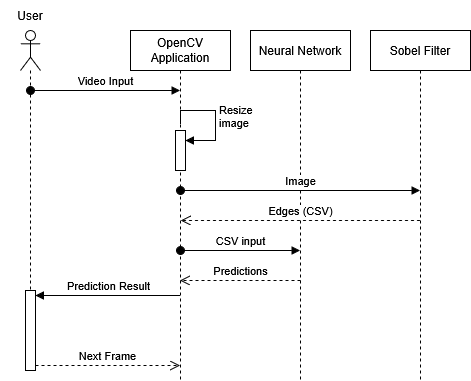
\includegraphics[width=.9\linewidth]{Introduction/2025-04-22_00-41-01_sequence_diagram.drawio.png}
\caption{\label{fig:org1e06527}Sequence Diagram of the application}
\end{figure}

\chapter{Sobel Filter}
\label{sec:org636f6fe}
The Sobel-Feldman operator (or simply Sobel filter) is a computer vision algorithm which can be used for edge detection. The filter takes a grayscale image as it's input and create another image emphasising the edges. This project uses the sobel filter as described in \citep{sobelop}. The operator is named after Irwin Sobel and Gary M. Feldman, who introduced the idea in 1968 at Stanford Artificial Intelligence Laboratory (SAIL). This filter uses the convolution operator to extract the edges from image by the change in magnitude.

\section{Convolution}
\label{sec:org5bcbe64}
Convolution is an operation which takes two matrices (an input and a kernel) and outputs another matrix which is of same size as the input matrix. It is the process of adding each element of the input to its local neighbors, weighted by the kernel. The convolution operation is denoted by *​. The operation usually uses a 3 \texttimes{} 3 sized kernel, but it is not necessary. Convolution is a simple to implement and fast operation to implement. But it is also very useful allowing for multiple useful filters. Some of the most simple and useful ones are Gaussian Blur, Sharpening and Sobel Filter (which we are using).

This project only uses the 3 \texttimes{} 3 sized kernels, this is done to make implementation simpler. This means in our case if the kernel is K and the input is I. Then the output O is given as

\[ O[x,y] = \sum_{i=0}^{2} \sum_{j=0}^{2} I[x + i - 1, y + j - 1] \times K[i,j] \]

So we can have our Matrix class as follows
\begin{minted}[breaklines=true,breakanywhere=true,linenos,frame=leftline]{cpp}
class Matrix
{
 public:
  int *data;
  int width;
  int height;
};
\end{minted}

\subsection{Border Pixels}
\label{sec:orga0ffe22}
But this function will not work for the pixels at the border of the input matrix. Since if we try to get the the value for border pixel [0, 0] we will need to get \(I[-1, -1]\), \(I[-1, 0]\), etc. pixels which do not exist since there are no pixels to the left. There are three common ways to solve this problem
\begin{itemize}
\item Filling with zeros, so that pixels outside the input are zero
\item Wrapping, the image is wrapped on all eight corners of the image
\item Mirroring, we mirror the image along the perimeter of the image
\end{itemize}

\begin{figure}[htbp]
\centering
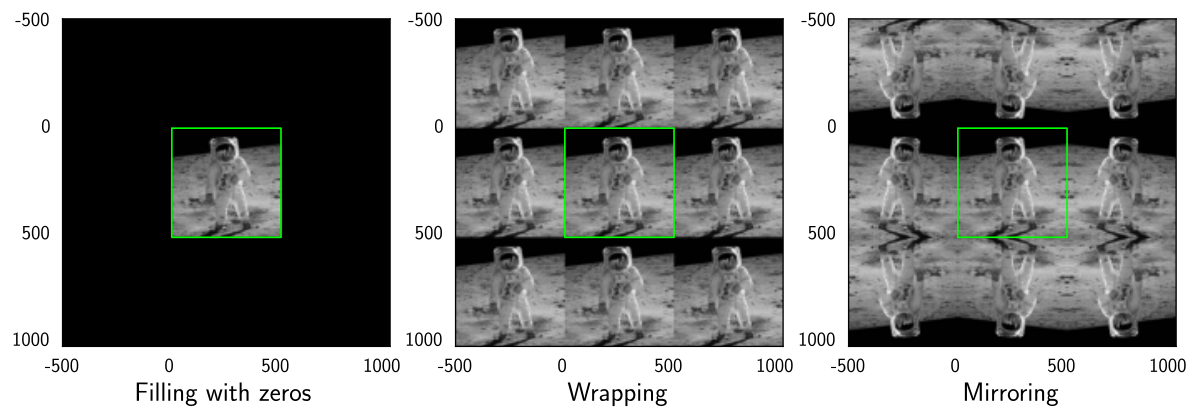
\includegraphics[width=.9\linewidth]{Sobel_Filter/2025-04-22_19-58-37_2025-04-22_19-55-12_boundaries-hypotheses.png}
\caption{\label{fig:orgddc0a97}The three ways to handle boundaries}
\end{figure}

This project will fill with zeros if we need a pixel outside the boundry of the image.

\begin{minted}[breaklines=true,breakanywhere=true,linenos,frame=leftline]{cpp}
int get(int w, int h)
{
  if(w >= this->width || w < 0 || h >= this->height || h < 0)
    return 0;
  return this->data[h * this->width + w];
}
\end{minted}

\subsection{Implementation}
\label{sec:org6eb35db}
Now that we know the definition of convolution and how to handle the edge cases, we can implement the this operation in code.
\begin{minted}[breaklines=true,breakanywhere=true,linenos,frame=leftline]{cpp}
Matrix convolute(Matrix kernel)
{
  uint8_t *opt = new uint8_t[this->width * this->height];
  Matrix output(opt, this->width, this->height);

  for(int w = 0; w < this->width; w++)
    {
      for(int h = 0; h < this->height; h++)
	{
	  int value =
	    kernel.get(0, 0) * this->get(w - 1, h - 1) +
	    kernel.get(0, 1) * this->get(w - 1, h - 0) +
	    kernel.get(1, 0) * this->get(w - 0, h - 1) +
	    kernel.get(1, 1) * this->get(w - 0, h - 0) +
	    kernel.get(0, 2) * this->get(w - 1, h + 1) +
	    kernel.get(1, 2) * this->get(w - 0, h + 1) +
	    kernel.get(2, 2) * this->get(w + 1, h + 1) +
	    kernel.get(2, 0) * this->get(w + 1, h - 1) +
	    kernel.get(2, 1) * this->get(w + 1, h - 0);
	  output.set(w, h, value);
	}
    }

  return output;
}
\end{minted}

\section{Formulation}
\label{sec:orgf9c6f85}
The sobel operator needs two convolution operations to detect the edges. The sobel operator works by calculating the change in image intensity, that is it works by calculating the difference in value of the value compared to its neighbors. The two convolution operations are to get the vertical changes and horizontal changes
\begin{enumerate}
\item Horizontal changes: This is represented as \(G_x\) and is calculated as
\[ G_x = \begin{bmatrix} -1 & 0 & +1\\ -2 & 0 & +2\\ -1 & 0 & +1 \end{bmatrix} \ast I \]
\item Vertical changes: This is represented as \(G_y\) and is calculated as
\[ G_y = \begin{bmatrix} -1 & -2 & -1\\ 0 & 0 & 0\\ +1 & +2 & +1 \end{bmatrix} \ast I \]
\end{enumerate}

We don't need the direction of the edge, we only need the magnitude. To calculate the magnitude, we will combine both the above results
\[ G = \sqrt{G_x^2 + G_y^2} \]

Using the Matrix class we implemented in previous section, we can implement this algorithm as
\begin{minted}[breaklines=true,breakanywhere=true,linenos,frame=leftline]{cpp}
Matrix sobel_x({1, 0, -1,
		2, 0, -2,
		1, 0 , -1}, 3, 3);
Matrix Gx = image.convolute(sobel_x);

Matrix sobel_y({1, 2, 1,
		0, 0, 0,
		-1, -2, -1}, 3, 3);
Matrix Gy = grayscale.convolute(sobel_y);
\end{minted}

The code to calculate magnitude is as follows
\begin{minted}[breaklines=true,breakanywhere=true,linenos,frame=leftline]{cpp}
double *magnitude = new double[width * height];
double max_magnitude = 0;
for(int i = 0; i < (width * height); i++)
  {
    double value = std::sqrt(Gx.data[i] * Gx.data[i] +
			     Gy.data[i] * Gy.data[i]);
    if (value > max_magnitude)
      max_magnitude = value;
    magnitude[i] = value;
  }
\end{minted}

Finally, we will output the image by converting the magnitude to an integer value between 0 and 255 by using the maximum magnitude.
\begin{minted}[breaklines=true,breakanywhere=true,linenos,frame=leftline]{cpp}
uint8_t *output = new uint8_t[width * height];
for(int i = 0; i < (width * height); i++)
  {
    output[i] = (magnitude[i] / max_magnitude) * 255;
  }
\end{minted}

\subsection{Result}
\label{sec:orgb613d2c}
The result of the sobel filter on one of the image from our dataset is shown in Figure \ref{fig:org1a46e5f}. Here, we have shown the output in form of a image by converting magnitude to an integer between 0 and 255. In the project, we work using magnitudes directly.

\begin{wrapfigure}{l}{0.5\textwidth}
\centering
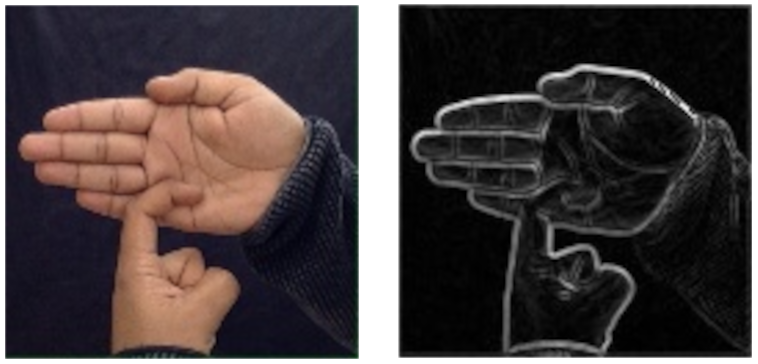
\includegraphics[width=0.48\textwidth]{Sobel_Filter/2025-04-28_02-44-20_edgeresult.png}
\caption{\label{fig:org1a46e5f}Result of sobel operator}
\end{wrapfigure}

\chapter{Neural Network}
\label{sec:orgb8eea2f}
A neural network is a type of machine learning model. It is inspired by the human brain, which is composed of neurons that form different pathways to process data and learn patterns. To mimic this behaviour, neural networks in coumputers are made of artificial neurons. An artificial neuron is a function which is conceived as a model of biological neuron in a neural network. An artificial neuron is the smallest unit of the Artificial Neural Network (ANN). The artificial neuron is based on how biological neurons work in human brain.

The artificial neurons are placed in layers to form our neural network. The input is passed to the first layer which is called the input layer, after which it moves forwards where are transformations are done on it by each neuron. This process is called the forward propagation. Eventually, the signal reaches the last layer called the output layer. The layers between input layer and output layers are called hidden layers. The number of artificial neurons in the input layer will depend on the size of our input. In our project, we have a 128 \texttimes{} 128 sized image, thus we will have 16,384 neurons in our input layer. We are making a recognizer, so number of neurons in output layer is number of classes. Thus our model will have 36 neurons in the output layer.

\section{Artificial Neurons}
\label{sec:org3fbc4aa}
The design of  artificial neurons is inspired by how biological neurons work. More precisely, it uses two types of behaviour from the biological neuron. There is excitatory potential and inhibitory potential for activation. So for every incoming signal, the neuron either increases it with excitatory potential or decreases it with inhibitory potential. This is copied in our artificial neuron as weights. These weights are multiplied with our inputs and can be used to increase or decrease the intensity of the different inputs. The appropriate value for these weights is calculated during training using a process called backpropagation.

\begin{figure}[htbp]
\centering
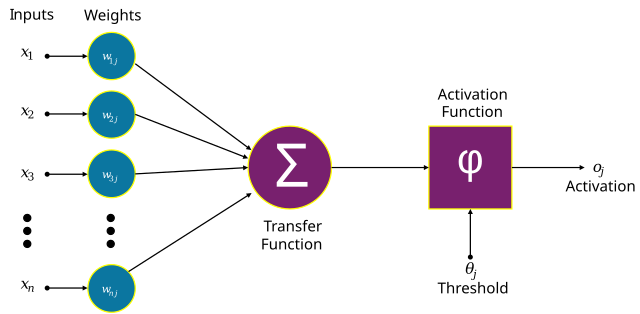
\includegraphics[width=.9\linewidth]{Neural_Network/2025-04-26_00-32-11_640px-Artificial_neuron_structure.svg.png}
\caption{\label{fig:orgde4f6ad}An artificial neuron}
\end{figure}

The structure of an artificial neuron is shown in Figure \ref{fig:orgde4f6ad}. A single neuron has multiple inputs it can take. This is shown in figure as variables \(x_1, x_2, x_3 ... x_n\). Every input to the neuron will have an associated weight. If we suppose the neuron number is \(j\) in the layer. We will represent the weights as \(w_{1j}, w_{2j}, w_{3j} ... w_{nj}\). Now we need to combine all the inputs. This is done by a transfer function, which is
summation in most models. Therefore, we will combine all the inputs as,

\[ x_1 w_{1j} + x_2 w_{2j} + x_3 w_{3j} + ... + x_n w_{nj} = \sum_{i=1}^{n} x_i w_{ij}\]

The next part of the neuron is the activation function. This function will take the result of the transfer function and produce the final output of the neuron. The need for activation function is to provide non-linearity. The transfer function only applies linear operations on the inputs. Having non-linear output allows our model to store relationships and patterns more efficiently. Some activation functions such as the ReLU function also help preventing signal saturation, a phenomenon where gradients become too small for learning.

Our model is only using a single activation function. It is the ReLU activation function. This function is very useful, specially in our project. This function helps to avoid the problem of vanishing gradients, which occurs in other activation functions. It is also simple to implement and computationally inexpensive. The one limitation of ReLU is that if inputs are consistently negetive, output will always be zero. In our project, we are using images with intensity of each pixel as input, this problem won't occur in our model. The graph of the ReLU function is shown in Figure \ref{fig:org78b14c4}.

\begin{figure}[htbp]
\centering
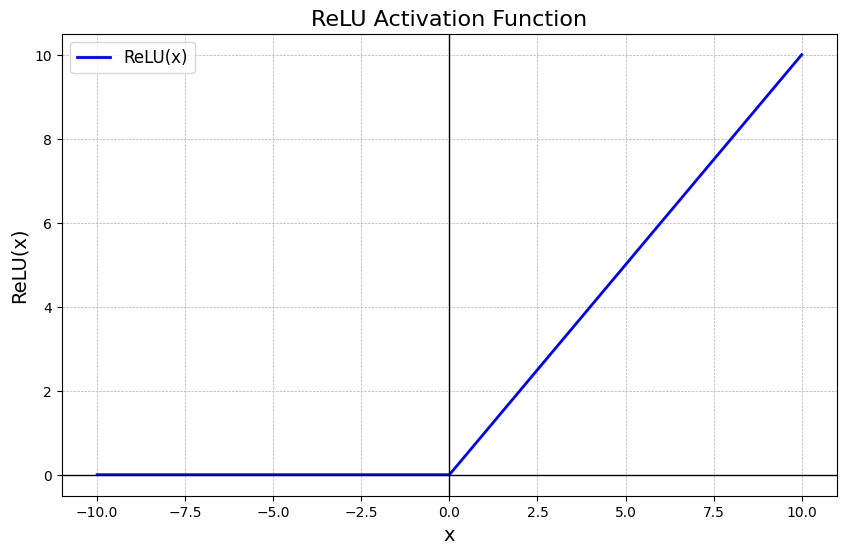
\includegraphics[width=.9\linewidth]{Neural_Network/2025-04-26_21-13-41_Relu-activation-function.png}
\caption{\label{fig:org78b14c4}ReLU Activation Function}
\end{figure}

The function is defined mathematically as
\[ ReLU(x) = \frac{x + |x|}{2} \]
But it is easier to implement in code by using the defition
\[ ReLU(x) = max(0, x) \]

\section{Training}
\label{sec:org5412e85}
The process of training in a neural network involves tweaking the weights associated with inputs of the neurons until we get expected results. In training and tweaking the weights, the model will learn the patterns in our input data. Thus, we will split our dataset into training data and testing data. The training data is used in the training process and the testing data is for testing our model. In our model, we have an 80 split for training and 20 for testing. The first step in training the model is choosing the loss function.

\subsection{Loss function}
\label{sec:org32a7fde}
The loss function (also called the cost function) is a function which shows how far our current predictions are from the actual answer. This allows us to automate the task of tweaking our weights in a way such that gets us better predictions, since we now only need to worry about minimizing the cost function and not worry about all of the neurons individually. There are multiple loss functions to choose from based on different use cases. A frequently used loss function is the Mean Square Error (MSE), but that function is better suited for regression. The loss function which is suitable for classification task is the Cross-Entropy loss function.

The Cross-Entropy loss function is used from \citep{lossfunc}. The cross-entropy loss increases as the predicted probability diverges from actual label. This function minimizes the cost when the signal of the predicted label is correct. It also increases the cost for when signals of other labels are high but this effect is weaker than previous. This is shown in Figure \ref{fig:orgedb8979} with the value of loss in y-axis and signal strength of predicted label is in x-axis.

\begin{figure}[htbp]
\centering
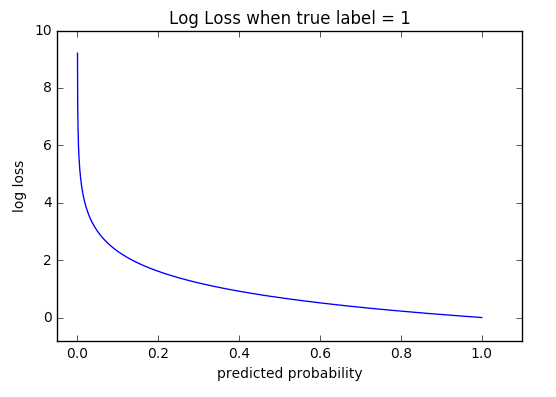
\includegraphics[width=.9\linewidth]{Neural_Network/2025-04-27_00-39-04_cross_entropy.png}
\caption{\label{fig:orgedb8979}Cross-Entropy loss function}
\end{figure}

The Cross-Entropy loss is calculated by the following equation. Here, \(M\) is the number of classes, \(y_i\) is the expected output of label \(i\) and \(p_i\) is the prediction.
\[ - \sum_{i = 1}^{M} y_{i} ln (p_{i}) \]

\subsection{Optimizer}
\label{sec:org6530441}
We now have a way to check the performance of the model, so we can use an optimizer which will find the appropriate weights to minimize the loss function. The most well known optimizer is the stochastic gradient descent (SDE). It is a variant of the gradient descent method, which is a general purpose algorithm which can be used to minimize any function.  It uses gradient (slope) to calculate the minima of the given loss function. According to \citep{gradientdescent}, the formula for gradient descent is

\[ W_{new} = W_{old} - \alpha \times \frac{\delta (Loss)}{\delta (W_{old})}\]

Where, \(W\) is the current value of the weight, and \(\alpha\) is the learning rate. Learning rate is the amount in which direction we move the weight. Choosing the correct learning rate is necessary for getting the minimum cost efficiently and correctly. If it is too high the optimization will take a very long time, having to do this for every weight will get very computationally expensive. Having it too high will cause the weights to jump around a lot, this causes it to never settle for the minima. This is show in Figure \ref{fig:orge336482} 

\begin{figure}[htbp]
\centering
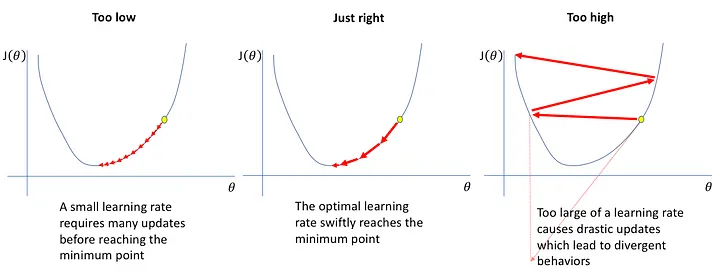
\includegraphics[width=.9\linewidth]{Neural_Network/2025-04-27_02-45-46_learning_rates.png}
\caption{\label{fig:orge336482}Choosing correct learning rate}
\end{figure}

This project uses Adaptive Gradient Descent (AdaGrad) which adaptively changes learning rate. This means that rather than being constant like we saw previously they are updated based sum of previous gradients squared.
\section{Implementation}
\label{sec:org6683db2}
The project uses TensorFlow to create and train the neural network. The model is trained on the Google Colab T4 (Tesla T4) compute unit. The model is trained on cloud and is then downloaded to be used in offline project. The following imports are used to train the model

\begin{minted}[breaklines=true,breakanywhere=true,linenos,frame=leftline]{python}
import pandas as pd 
import numpy as np
import tensorflow as tf
from sklearn.model_selection import train_test_split
from google.colab import drive
\end{minted}

We process the dataset using sobel filter and save the results in a csv file in the our drive, this is then loaded into the cloud. We also split the dataset into training and testing data.

\begin{minted}[breaklines=true,breakanywhere=true,linenos,frame=leftline]{python}
data = pd.read_csv('/content/drive/MyDrive/isl.csv', header=None)
X, Y = data.iloc[:,0:16384].values, data[16384].values
X_train, X_test, Y_train, Y_test = train_test_split(X,Y,test_size=0.2)
\end{minted}

After the dataset is loaded, we will make our model. This model has three layers, input layer has 16,384 neurons and uses the ReLU activation function. The second layer has 8,174 neurons and also uses the ReLU activation function. This hidden layer has the number of neurons chosen to be between neurons in input layer and those in output layer. The output layer is a layer with 36 neurons. This is built in tensorflow as

\begin{minted}[breaklines=true,breakanywhere=true,linenos,frame=leftline]{python}
 model = tf.keras.Sequential([
   tf.keras.layers.Dense(128*128, activation='relu'),
   tf.keras.layers.Dense(8174, activation='relu'),
   tf.keras.layers.Dense(36)
])
\end{minted}

To train this model we need to call the compile and fit methods as shown

\begin{minted}[breaklines=true,breakanywhere=true,linenos,frame=leftline]{python}
model.compile(optimizer='adagrad', metrics=['accuracy'],
	      loss=tf.keras.losses.SparseCategoricalCrossentropy(from_logits=True))
model.fit(X_train, Y_train, epochs=5)
\end{minted}

Now, we can check the accuracy of our model using the testing data. The output for this is shown in Figure \ref{fig:org6091b20}. 

\begin{figure}[htbp]
\centering
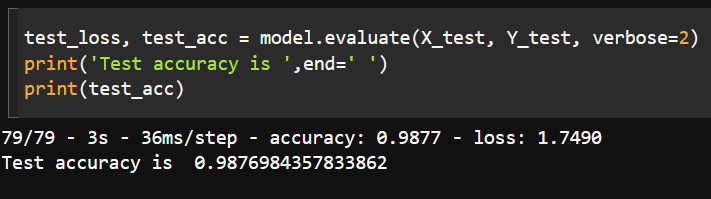
\includegraphics[width=.9\linewidth]{Neural_Network/2025-04-28_01-55-46_accuracy_of_model.png}
\caption{\label{fig:org6091b20}Accuracy of the model}
\end{figure}

The common way to show the accuracy of a model is to use a confusion matrix. It has the true labels in the Y-axis and predicted label in X-axis and data is shown in form of a matrix. Each cell shows the percent of time the model makes the prediction for the given label corresponding true label. Thus if model is has high accuracy, the diagonal will have should be high. The confusion matrix of our model is shown in Figure \ref{fig:orgf7e9dcb}. We can see that our model shows confusion for 'U', '7', '6' and '4' but otherwise has very high accuracy.

\begin{figure}[htbp]
\centering
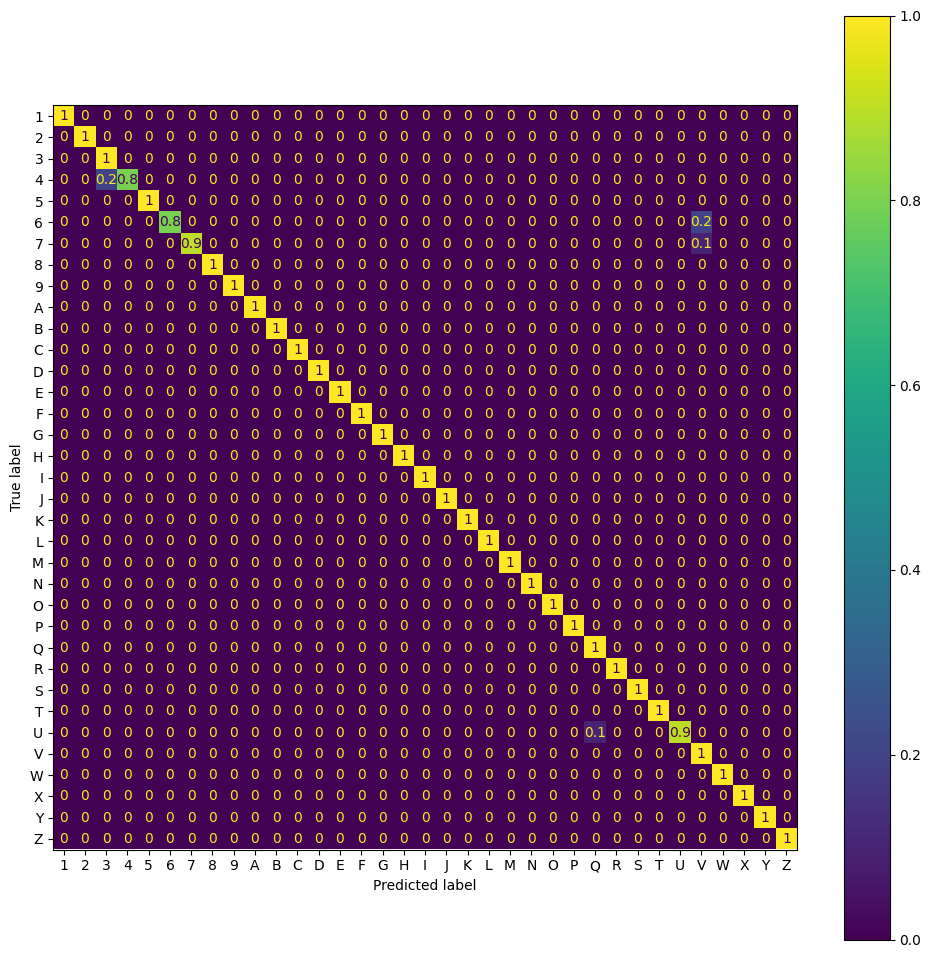
\includegraphics[width=.9\linewidth]{Neural_Network/2025-04-27_03-38-55_confusion_matrix.png}
\caption{\label{fig:orgf7e9dcb}The confusion matrix}
\end{figure}

\chapter{OpenCV Application}
\label{sec:orgcd23868}
The final component of this project is the OpenCV application which will take the input from the user. It takes the video from webcam as the input. It will then pass the input through our sobel filter. It will finally use the model which we trained to give a prediction. We can predict using the \(model.predict\) method. The result of this function is shown in Figure \ref{fig:org92a7249}. This returns an array of predictions, where every index represents a different label. The index with the largest signal is the label which our model predicted.

\begin{figure}[htbp]
\centering
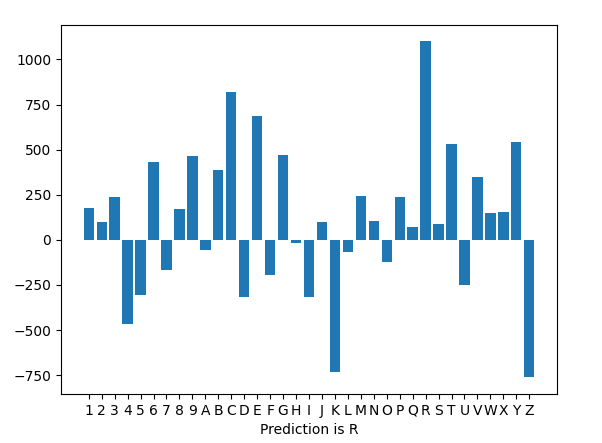
\includegraphics[width=.9\linewidth]{OpenCV_Application/2025-04-27_15-22-20_Screenshot 2025-03-18 121040.png}
\caption{\label{fig:org92a7249}The result of prediction}
\end{figure}

\section{Implementation}
\label{sec:org6987be3}
The first step is to setup the openCV loop. This loop is called every frame of the video
\begin{minted}[breaklines=true,breakanywhere=true,linenos,frame=leftline]{python}
import pandas as pd
import tensorflow as tf
import numpy as np
import cv2

import subprocess
from io import StringIO

# Main loop
capture = cv2.VideoCapture(0)
frame_number = 0
current_prediction = "Waiting..."
while(True):
    ret, frame = capture.read()
    cv2.putText(frame, current_prediction,
		(10,20), cv2.FONT_HERSHEY_COMPLEX,
		1,( 255, 0, 0),2,cv2.LINE_AA)
    cv2.imshow("Press Q to close", frame)

    if (cv2.waitKey(1) == ord('q')):
	break

capture.release()
cv2.destroyAllWindows()
\end{minted}

Now, we need to get a square region in the middle of the frame where we can get the input. Thus we will need some global variables that will define the region
\begin{minted}[breaklines=true,breakanywhere=true,linenos,frame=leftline]{python}
# Region properties
REGION_TOP_LEFT = (272, 272)
REGION_SIZE = (512, 512)
REGION_BOUNDRY_COLOR = (255, 0, 0)
REGION_BOUNDRY_SIZE = 3

region_bottom_right = (REGION_TOP_LEFT[0] + REGION_SIZE[0],
		       REGION_TOP_LEFT[1] + REGION_SIZE[1])
\end{minted}

Now, in our main loop we will add the following line to put the region in our frame after the cv2.putText
\begin{minted}[breaklines=true,breakanywhere=true,linenos,frame=leftline]{python}
cv2.rectangle(frame, REGION_TOP_LEFT, region_bottom_right,
	      REGION_BOUNDRY_COLOR, REGION_BOUNDRY_SIZE)
\end{minted}

Finally, in our we can get the region after the cv2.imshow call to get the region and write it to an output.jpg
\begin{minted}[breaklines=true,breakanywhere=true,linenos,frame=leftline]{python}
if frame_number % 120 == 0:
  # Getting region
  region = frame[REGION_TOP_LEFT[0]:region_bottom_right[0],
		 REGION_TOP_LEFT[1]:region_bottom_right[1]]
  region = cv2.cvtColor(region, cv2.COLOR_BGR2GRAY)
  region = cv2.resize(region, (128, 128))
  region = cv2.flip(region, 1)
  cv2.imwrite("output.jpg", region)
\end{minted}

After we have written our output image, we can then give it to the sobel filter. To run other processes, we use the python subprocess module.
\begin{minted}[breaklines=true,breakanywhere=true,linenos,frame=leftline]{python}
opt = subprocess.check_output("./sobel.exe " + "output.jpg")
inpt = pd.read_csv(StringIO(opt.decode('utf-8')[0:-1]), header=None)
\end{minted}

Since we now have data in form of numpy array, we can pass the values to the model to get our predictions and change the current predictions accordingly.
\begin{minted}[breaklines=true,breakanywhere=true,linenos,frame=leftline]{python}
predictions = model.predict(inpt.values)
current_prediction = "Prediction is " +
		     characters_label[np.argmax(predictions)]
\end{minted}

\chapter{Conclusion}
\label{sec:orgb320f12}
In this chapter, we will present the results we got in this project in brief. The sobel filter is the first major component of this project. Since this is written in C++, this is very fast and computationally efficient. It is also very portable because the main logic is written in pure C++ and library to read and write images are the stb single file libraries \citep{stblibraries} which are very small and cross platform. The filter being implemented in a system programming language also means it is easy to integrate with other languages.

To classify our images after applying the sobel operator, we have use an Artificial Neural Network (ANN) with three layers. The model supports inputs of size 128 \texttimes{} 128. The first layer has 16,384 neurons for input and is using ReLU activation function. The second layer which is the hidden layer of our model, has 8,174 neurons and also uses the ReLU activation function. The final layer which is the output layer has 36 neurons for the number of classes we need to recognize. We use the cross-entropy loss function because it works well with classification tasks, especially with high number of classes. We use the AdaGrad algorithm for optimization of the loss function. This is a variant of the Gradient Descent in which learning rates are adjusted during training. In our testing data, this gave us an accuracy of 98.77\%  as seen in Figure \ref{fig:org6091b20} this may be lower for other more general datasets and needs more testig with varied inputs.

The final component of our project is the openCV application which ties the other two parts together, allowing us to take input from real-time video and pass it through other two components. It will also tell the prediction to the user. This application has the most scope for work in the future. This component currently rescales the input, applies grayscale (though this part is not necessary since the sobel filter application can do it) and then saves the image. Then it calls sobel filter application to convert the image to csv output, this is data is given to the model which produces the final prediction.

\chapter{Future Scope}
\label{sec:orge515fae}
There are many future avenues for exploration, several compelling directions emerge, aligning seamlessly with the trajectory of this project and its uses for use by general public. Firstly, we can devle deeper into the edge detection where we can upgrade from a simple sobel filter to canny edge detection. This algorithm works after sobel filter to further select only the most prominent edges. This will help in getting better accuracy when working on real-time input like video, because most modern cameras usually focus on the foreground effectively making edges of the focus (hands) more prominent. We can go further and add a way to remove the background from our input. This would required another suitable algorithm or model which can detect the background and remove it.

The neural network can be upgraded to a Convolution Neural Network (CNN). These networks are better suited for computer vision tasks than traditional Neural Network which we have used in this project. Increasing the quality of the dataset, with more varied images which the network can train on. It would also be ideal if these images could have more noise in the background so that we could train the model to only isolate the hands.

The frontend application needs the most work in the future, if this project is to be used for gesture detection in true-to-life setting. The current implementation relies on OpenCV, but we are not using all of the capabilities of the library. It was chosen since it was appropriate for the scope of this project, but switching to another library which is lighter and can allow us to work with camera directly will significantly improve performance. Alternatively, we could also use OpenCV to do more difficult tasks such as the canny edge detection mentioned before. This would make the use of such a large library appropriate. The fontend also needs to be more user friendly and intuitive to use.

In essence, the future holds boundless opportunities for advancing the field of sign language recognition through interdisciplinary collaboration, innovative technologies, and a steadfast commitment to excellence. By embracing these opportunities and staying attuned to emerging trends and challenges, we can continue to push the boundaries of what's achievable, driving innovation and shaping the future of computer vision.
\bibliographystyle{abbrv}
\bibliography{d:/Projects/Indian-Sign-Language-Recognizer/report/bibliography}
\end{document}